\documentclass[11pt]{article}
\usepackage[margin=1in]{geometry}
\usepackage[T1]{fontenc}
\usepackage[utf8]{inputenc}
\usepackage{lmodern,microtype}
\usepackage{amsmath,amssymb,amsthm,mathtools,bm}
\usepackage{booktabs,tabularx,array}
\usepackage{graphicx}
\usepackage[dvipsnames]{xcolor}
\usepackage{enumitem,caption,float,url}
\usepackage{hyperref}
\usepackage[nameinlink,noabbrev]{cleveref}
\hypersetup{colorlinks=true,linkcolor=MidnightBlue,citecolor=BrickRed,
urlcolor=RoyalBlue,pdftitle={From Polygonal Quantum Control to an Emergent Local Metric},
pdfauthor={QBist Spacetime Reinforcement-Learning Project}}
\setlength{\emergencystretch}{3em}
\setcounter{tocdepth}{2}
\newtheorem{theorem}{Theorem}[section]
\newtheorem{proposition}[theorem]{Proposition}
\newtheorem{corollary}[theorem]{Corollary}
\theoremstyle{definition}\newtheorem{definition}[theorem]{Definition}
\theoremstyle{remark}\newtheorem{remark}[theorem]{Remark}
\newcommand{\C}{\mathbb C}
\newcommand{\R}{\mathbb R}
\newcommand{\Z}{\mathbb Z}
\newcommand{\E}{\mathbb E}
\newcommand{\tr}{\operatorname{tr}}
\newcommand{\conv}{\operatorname{conv}}
\newcommand{\rank}{\operatorname{rank}}
\newcommand{\cE}{\mathcal E}
\newcommand{\ket}[1]{\lvert #1\rangle}
\newcommand{\bra}[1]{\langle #1\rvert}
\newcommand{\braket}[2]{\langle #1\mid #2\rangle}
\newcommand{\proj}[1]{\lvert #1\rangle\!\langle #1\rvert}
\newcommand{\norm}[1]{\left\lVert #1\right\rVert}
\newcommand{\abs}[1]{\left\lvert #1\right\rvert}

\title{\textbf{From Polygonal Quantum Control to an Emergent Local Metric}\\[0.5em]
\large Finite-direction obstructions, nonorthogonal qutrit localization,\\
and a route to continuous predictive geometry}
\author{QBist Spacetime Reinforcement-Learning Project}
\date{August 11, 2026}

\begin{document}
\maketitle

\begin{abstract}
Can ordinary two-dimensional space arise as the geometry of goals for an
agent controlling a quantum system whose Hilbert space has only three
dimensions? Earlier exact constructions answer the cardinality question
affirmatively: a qubit or qutrit has continuously many nonorthogonal states,
and priced displacement instruments can make a finite goal set have exact
Euclidean distances. Those constructions do not yet explain locality because
they include an action tailored to every desired displacement.

This paper studies the stronger local problem. We construct a
translation-covariant qutrit phase orbit and restrict the agent to one finite,
goal-independent catalog of local binary Kraus instruments. We prove that
retry instruments reduce exactly to a weighted word metric and that the
large-scale unit ball is the convex hull of normalized primitive velocities.
A fixed finite catalog therefore induces a polygonal Finsler norm, not a
Euclidean norm. If its largest angular gap is \(\Delta_{\max}\), the worst
asymptotic excess is \(\sec(\Delta_{\max}/2)-1\); approximately uniform
\(K\)-direction catalogs converge only as \(O(K^{-2})\).

Deterministic inverse-design experiments confirm this obstruction beyond the
fitting region. Held-out Euclidean relative RMSE falls from \(30.03\%\) with
four directions to \(3.85\%\) with eight and \(1.62\%\) with 32. The
32-direction geometry has two-dimensional MDS stress \(0.0289\), but retains
Schoenberg negative-eigenmass fraction \(0.082\), preventing an exact
Euclidean interpretation. Sixteen nominal directions do no better than eight
because their new moves are Bellman-dominated.

We then hide the initial position on a nine-state nonorthogonal qutrit phase
grid and derive an exact Bayesian quantum filter for weak covariant
measurements. In 60,000 episodes, informative measurements improve
preparation-label navigation above the null value \(1/9\), while known-start
navigation is exact. Nevertheless, a sharp measurement identifies the initial
label with probability only \(1/3\) while preparing a present state that can
be translated to the target with fidelity one. Historical localization and
present-state control are inequivalent. Together the results identify a base
action geometry and an epistemic quantum fiber, and motivate a next model with
continuous qutrit controls, quadratic effort, and a learned predictive atlas.
\end{abstract}

\tableofcontents
\newpage

\section{Introduction}
\label{sec:introduction}

\subsection{Space as a geometry of achievable goals}

The working hypothesis is operational: an agent need not begin with physical
space as a primitive. What it directly encounters is a collection of goals
and interventions. Some goals require few reliable interventions; others
require longer, riskier, or more information-intensive strategies. This
induces a \emph{hodological} geometry---a geometry of routes and goal
difficulty---before coordinates are assigned.

Let \(z\) be an operational state, \(g\) a goal, and \(\tau_g\) its first
hitting time. For a policy \(\pi\),
\begin{equation}
d_\pi(z,g)=\E_\pi\left[
\sum_{t=0}^{\tau_g-1}c(z_t,a_t)\,\middle|\,z_0=z\right].
\label{eq:policy-cost}
\end{equation}
Optimizing gives \(D(z,g)=\inf_\pi d_\pi(z,g)\). In general \(D\) can be
directed, nonmetric, and high-dimensional. Ordinary space would be a special
regime in which many place-like goals have nearly symmetric costs, admit a
low-distortion common embedding, and support local homogeneous displacements.
This uses the machinery of reinforcement learning (RL), partially observed
control, and stochastic shortest paths \cite{bellman1957,puterman1994,
sutton2018,kaelbling1998}, but reverses the usual interpretation: values are
evidence for whether space should emerge, not merely tools for navigation in a
space assumed in advance.

\subsection{Low Hilbert dimension is not low goal cardinality}

A \(d\)-dimensional Hilbert space has at most \(d\) mutually orthogonal pure
states but continuously many distinct density operators. Orthogonality limits
perfect one-shot discrimination, not controlled-orbit size. Nine goals need
not be nine basis states in a nine-dimensional position register. They can be
nine nonorthogonal qutrit states or nine sequence-goal conditions.

This freedom has a danger: an unrestricted classical goal automaton can
manufacture any finite graph while the quantum system remains idle. Physical
Hilbert dimension, predictive-state dimension, and controller-memory
dimension must be distinguished. Exact state preparation must also be
distinguished from localization, because measurement can prepare an
easy-to-control state while erasing its origin.

\subsection{The locality problem}

An earlier exact benchmark supplies one retry action for each source--goal
difference \(\delta\), with success probability
\(p_\delta=1/\norm{\delta}_2\). Its expected attempt count is exactly
\(\norm{\delta}_2\). This proves possibility, but explicitly puts Euclidean
length into goal-sized macro-actions. The stronger question is:
\begin{quote}
\emph{Can a fixed, small, translation-covariant family of local qutrit
interventions generate an ordinary metric by composition, including on
directions and distances not used to tune it?}
\end{quote}
The answer is approximately yes and exactly no for fixed finite headings.
The obstruction is geometric: additive local control with finitely many
velocities has a polygonal unit ball.

\subsection{Contributions}

We provide:
\begin{enumerate}[leftmargin=2em]
\item an exact reduction from random-unitary retry instruments to weighted
word metrics and a proof of their polygonal stable norms;
\item deterministic inverse design for four qutrit control stencils, tested on
held-out displacements with Bellman, locality, MDS, and Schoenberg diagnostics;
\item an exact Bayesian quantum filter for weak localization on a nine-state
nonorthogonal qutrit phase orbit;
\item a separation between historical-label goals and present-state goals;
\item a concrete continuous-control predictive-atlas research program.
\end{enumerate}

\section{Quantum and reinforcement-learning background}
\label{sec:background}

\subsection{Quantum instruments}

A state on \(\mathcal H\cong\C^d\) is a positive semidefinite matrix \(\rho\)
with \(\tr\rho=1\). For action \(a\) and observed outcome \(o\), a quantum
instrument has completely positive branches
\begin{equation}
\cE_o^a(\rho)=\sum_kK_{o,k}^a\rho K_{o,k}^{a\dagger},
\qquad
\sum_{o,k}K_{o,k}^{a\dagger}K_{o,k}^a=I.
\label{eq:instrument}
\end{equation}
The probability and conditional state are
\begin{equation}
p(o\mid\rho,a)=\tr\cE_o^a(\rho),\qquad
\rho'=\frac{\cE_o^a(\rho)}{p(o\mid\rho,a)}.
\label{eq:born}
\end{equation}
Thus a measurement both informs and disturbs. This is the key feature absent
from a classical likelihood table \cite{kraus1983,nielsen2010,wiseman2010}.

A random-unitary retry instrument is
\begin{equation}
K_{\rm s}=\sqrt p\,U,\qquad K_{\rm f}=\sqrt{1-p}\,I.
\label{eq:retry}
\end{equation}
Its success probability is state independent; failure leaves the state
unchanged; success applies \(U\).

\subsection{Bellman optimality}

In a finite Markov decision process, the shortest-path value for goal \(g\)
obeys
\begin{equation}
V_g(g)=0,\qquad
V_g(s)=\min_a\left[c(s,a)+\sum_{s'}P(s'\mid s,a)V_g(s')\right].
\label{eq:bellman}
\end{equation}
The equality says that an optimal plan is consistent under one-step
decomposition. When the hidden quantum state is not observed, a policy depends
on the action--outcome history. A Bayesian belief or learned recurrent state
must retain distinctions that matter to future outcome distributions and
goals. Predictive-state representations formalize this operational criterion
\cite{littman2002}.

\subsection{Sequence goals and memory}

A sequence goal is a language over action--outcome symbols. A finite automaton
updates \(q_{t+1}=\delta(q_t,a_t,o_t)\); the Markov state is then
\((\rho_t,q_t)\). This allows more goals than orthogonal quantum states, but
the automaton memory is an additional resource. An exact unbounded
\(\Z^2\) displacement language needs counters or an episode horizon.

\subsection{Metric and Euclidean tests}

An optimal cost is an ordinary metric only if it is symmetric, positive, and
satisfies the triangle inequality. For Euclidean compatibility, define
\begin{equation}
J=I-\frac1n\bm1\bm1^\top,\qquad
B=-\frac12JD^{\circ2}J.
\label{eq:schoenberg}
\end{equation}
Schoenberg's theorem says that \(D\) embeds exactly in Euclidean space iff
\(B\succeq0\), and in \(\R^k\) iff additionally
\(\rank B\le k\) \cite{schoenberg1935,borg2005}.
Metric MDS seeks coordinates minimizing
\begin{equation}
\operatorname{Stress}_k=
\sqrt{\frac{\sum_{i<j}(\norm{x_i-x_j}_2-D_{ij})^2}
{\sum_{i<j}D_{ij}^2}}.
\label{eq:stress}
\end{equation}
Low stress is useful but does not replace the exact spectral test
\cite{kruskal1964}. Spatial dynamics also require local, translation-consistent
action increments, not merely a pleasing embedding.

\section{Translation-covariant qutrit controls}
\label{sec:qutrit}

\subsection{Equilateral phase encoding}

Define reciprocal vectors
\begin{equation}
q_0=(1,0),\quad
q_1=(-1/2,\sqrt3/2),\quad
q_2=(-1/2,-\sqrt3/2).
\end{equation}
They obey
\[
\sum_nq_n=0,\qquad \frac13\sum_nq_nq_n^\top=\frac12I_2.
\]
Encode \(x\in\R^2\) as
\begin{equation}
\ket{\psi(x)}=\frac1{\sqrt3}\sum_{n=0}^2
e^{i\kappa q_n\cdot x}\ket n,\qquad \kappa=0.15.
\label{eq:phase-encoding}
\end{equation}
For displacement \(a\),
\begin{equation}
U_a=\operatorname{diag}\left(
e^{i\kappa q_0\cdot a},e^{i\kappa q_1\cdot a},
e^{i\kappa q_2\cdot a}\right)
\end{equation}
satisfies \(U_a\ket{\psi(x)}=\ket{\psi(x+a)}\) exactly. The same action
translates every point; covariance is supplied by the group law rather than
learned separately at each site.

\subsection{Local projective geometry}

The Fubini--Study distance is
\[
d_{\rm FS}(x,y)=\arccos\abs{\braket{\psi(x)}{\psi(y)}}.
\]
Expansion around \(dx=0\), using the reciprocal-vector identities, gives
\begin{equation}
d_{\rm FS}(x,x+dx)^2=\frac{\kappa^2}{2}\norm{dx}_2^2
+O(\norm{dx}_2^4).
\label{eq:fs-local}
\end{equation}
The qutrit orbit is locally isotropic. It is also compact and recurrent, so
its ambient distance cannot equal an unbounded homogeneous history-space
distance globally \cite{bengtsson2017}.

\subsection{Local Kraus attempts}

For each allowed stencil vector \(a\), use
\begin{equation}
K_{a,\rm s}=\sqrt{p_a}\,U_a,\qquad
K_{a,\rm f}=\sqrt{1-p_a}\,I_3.
\label{eq:local-kraus}
\end{equation}
Every attempt costs one. Parameters are shared under sign changes and
coordinate permutations. Optimization can choose a cost for each primitive
symmetry class but cannot introduce a goal- or site-specific action.

\section{The finite-direction theorem}
\label{sec:theory}

\subsection{Exact reduction to a word metric}

Let \(S\subset\Z^2\setminus\{0\}\) be finite, symmetric, and spanning. Give
action \(v\) attempt cost \(c_v>0\) and success probability \(p_v>0\), and
define \(\ell_v=c_v/p_v\).

\begin{proposition}[Exact local hodology]
\label{prop:word}
If failure leaves the operational state unchanged and supplies no additional
hidden-state information, then
\begin{equation}
D_S(x,g)=\inf\left\{\sum_{k=1}^n\ell_{v_k}:
v_k\in S,\ \sum_{k=1}^nv_k=g-x\right\}.
\label{eq:word}
\end{equation}
\end{proposition}

\begin{proof}
Retrying \(v\) until success takes a geometric number of attempts with mean
\(1/p_v\), so every successful word is achievable at expected cost
\(\sum_k\ell_{v_k}\). Let \(V\) be the right side. Its triangle inequality
gives \(V(x)-V(x+v)\le c_v/p_v\). Therefore
\[
c_v+(1-p_v)V(x)+p_vV(x+v)\ge V(x).
\]
No first action or adaptive continuation can beat \(V\). Positivity and
reachability make it the minimal nonnegative Bellman solution.
\end{proof}

\subsection{Exact Euclidean rays}

\begin{proposition}[Ray criterion]
\label{prop:ray}
If \(\ell_v=\norm v_2\), then
\[
D_S(0,z)=\norm z_2
\]
iff \(z\) is a sum of available vectors all lying on its oriented ray.
\end{proposition}
\begin{proof}
For every word summing to \(z\),
\[
\sum_k\norm{v_k}_2\ge\norm{\sum_kv_k}_2=\norm z_2.
\]
Strict convexity makes equality equivalent to all nonzero summands being
nonnegative collinear vectors.
\end{proof}

\begin{corollary}
No fixed finite catalog is exactly Euclidean on all of \(\Z^2\). Exactness on
a radius-\(R\) square needs a primitive action ray for every coprime pair
\((a,b)\) with \(0\le a,b\le R\), hence \(O(R^2)\) headings.
\end{corollary}

\subsection{Polygonal stable norm}

Define
\begin{equation}
P_S=\conv\{v/\ell_v:v\in S\},\qquad
\norm x_{P_S}=\inf\{\lambda>0:x\in\lambda P_S\}.
\label{eq:gauge}
\end{equation}

\begin{theorem}[Stable local-control norm]
\label{thm:stable}
If \(S\) generates \(\Z^2\), then
\[
\lim_{n\to\infty}\frac{D_S(0,nz)}n=\norm z_{P_S}.
\]
For finite \(S\), this is a polygonal norm and cannot equal the Euclidean norm
in every direction.
\end{theorem}
\begin{proof}
The gauge has the linear-program form
\[
\norm x_{P_S}=\inf_{\alpha_v\ge0}
\left\{\sum_v\alpha_v\ell_v:\sum_v\alpha_vv=x\right\}.
\]
Every integer word is feasible, giving the lower bound. Conversely, multiply
an optimal fractional decomposition by \(n\), round its coefficients, and
correct the bounded lattice residue using a fixed generating subset. Thus
\[
n\norm z_{P_S}\le D_S(0,nz)\le n\norm z_{P_S}+C_z.
\]
Division by \(n\) proves convergence. A finite convex hull is a polygon, while
the Euclidean unit disk has infinitely many extreme points.
\end{proof}
This is a flat Finsler continuum limit \cite{bao2000,burago2001}. Refining the
site spacing with fixed headings samples the polygon more densely but does not
make it circular.

\subsection{Angular error and exact examples}

If \(\ell_v=\norm v_2\) and \(\Delta_{\max}\) is the largest angular gap
between adjacent headings, chord geometry gives
\begin{equation}
1\le\frac{\norm x_{P_S}}{\norm x_2}\le
\sec(\Delta_{\max}/2).
\label{eq:angular}
\end{equation}
For \(K\) evenly spaced oriented directions,
\[
\sec(\pi/K)-1=\frac{\pi^2}{2K^2}+O(K^{-4}).
\]

Four axial moves give the Manhattan norm. Adding diagonals of cost \(\sqrt2\)
gives the octile norm
\begin{equation}
D_8(a,b)=A+(\sqrt2-1)B,\quad
A=\max(\abs a,\abs b),\quad B=\min(\abs a,\abs b).
\label{eq:octile}
\end{equation}
Its asymptotic worst excess is \(0.0823922\); at \((2,1)\) the excess is
\[
\frac{1+\sqrt2}{\sqrt5}-1=0.0796691.
\]
Adding all knight headings \((\pm2,\pm1)\) and permutations can make a
\(3\times3\) patch exact if their costs are Euclidean, but larger patches
contain missing slopes. Small-patch exactness does not prove asymptotic
Euclidean geometry.

\section{Control inverse design and evaluation}
\label{sec:control-method}

\subsection{Repertoires}

\begin{table}[htbp]
\centering
\caption{Fixed local repertoires. Locality ratio is maximum primitive step
divided by held-out evaluation radius 12.}
\label{tab:repertoires}
\begin{tabular}{lrrrr}
\toprule
Name & directions & parameters & max.\ step & locality ratio\\
\midrule
D4 & 4 & 1 & 1.000 & 0.083\\
D8 & 8 & 2 & 1.414 & 0.118\\
D16 & 16 & 3 & 2.236 & 0.186\\
D32 & 32 & 5 & 3.606 & 0.300\\
\bottomrule
\end{tabular}
\end{table}
D4 has axes, D8 adds diagonals, D16 adds knight headings, and D32 adds
primitive slopes with maximum coordinate three. The catalog is fixed before
source and goal are supplied.

\subsection{Targets, optimization, and held-out test}

Translation covariance reduces planning to
\begin{equation}
V(0)=0,\qquad V(x)=\min_{a\in\mathcal A}\{c_a+V(x-a)\},
\label{eq:displacement-bellman}
\end{equation}
solved exactly by Dijkstra's algorithm. The targets are Euclidean distance and
\[
\widetilde d_{\rm FS}(0,x)=\frac{\sqrt2}{\kappa}
\arccos\abs{\braket{\psi(0)}{\psi(x)}}.
\]
The latter agrees with Euclidean distance infinitesimally but contains compact
projective curvature at finite radius.

A deterministic projected coordinate search minimizes mean squared relative
error on all 48 nonzero integer displacements within radius four. Costs begin
at \(1.18\norm a_2\), satisfy \(c_a\ge1\), and share square symmetries. All
392 displacements with radii \(4<r\le12\) are held out. Evaluation reports
quantum validity, Bellman residual, held-out errors, radial anisotropy, MDS
stress, Schoenberg spectrum, and locality. These metrics prevent a persuasive
plot from substituting for geometric evidence.

\section{Control results}
\label{sec:control-results}

All validity checks close at numerical precision: maximum Kraus completeness
residual \(2.22\times10^{-16}\), covariance residual
\(1.67\times10^{-16}\), and Bellman residual \(1.78\times10^{-15}\).

\begin{table}[htbp]
\centering
\caption{Held-out performance on 392 displacements. Errors are relative to
the named target.}
\label{tab:control}
\begin{tabular}{llrrr}
\toprule
Target & catalog & RMSE & mean error & max.\ abs.\ error\\
\midrule
Euclidean & D4 & 0.3003 & 0.2719 & 0.4142\\
Euclidean & D8 & 0.0385 & 0.0220 & 0.0607\\
Euclidean & D16 & 0.0385 & 0.0220 & 0.0607\\
Euclidean & D32 & \textbf{0.0162} & 0.0022 & 0.0491\\
\addlinespace
scaled FS & D4 & 0.3337 & 0.3063 & 0.4954\\
scaled FS & D8 & 0.0614 & 0.0484 & 0.1240\\
scaled FS & D16 & 0.0614 & 0.0484 & 0.1240\\
scaled FS & D32 & \textbf{0.0365} & 0.0276 & 0.0898\\
\bottomrule
\end{tabular}
\end{table}

D8 is the best locality--accuracy compromise. Its diagonal expected cost is
\(1.32836\), or success probability \(0.75281\). It is slightly cheaper than
\(\sqrt2\), balancing finite-disk relative errors rather than exactly matching
the asymptotic circle.

D16 does not improve on D8. Its knight cost remains \(2.63856\), above a
cheaper diagonal-plus-axial composite, so the added velocity lies inside the
effective hull. Action count alone is not geometric expressivity; only exposed
hull vertices matter. D32 activates a \((3,1)\) heading with cost
\(3.16229\), close to \(\sqrt{10}\), and achieves \(1.62\%\) held-out RMSE,
at the cost of a longer maximum primitive.

\begin{figure}[p]
\centering
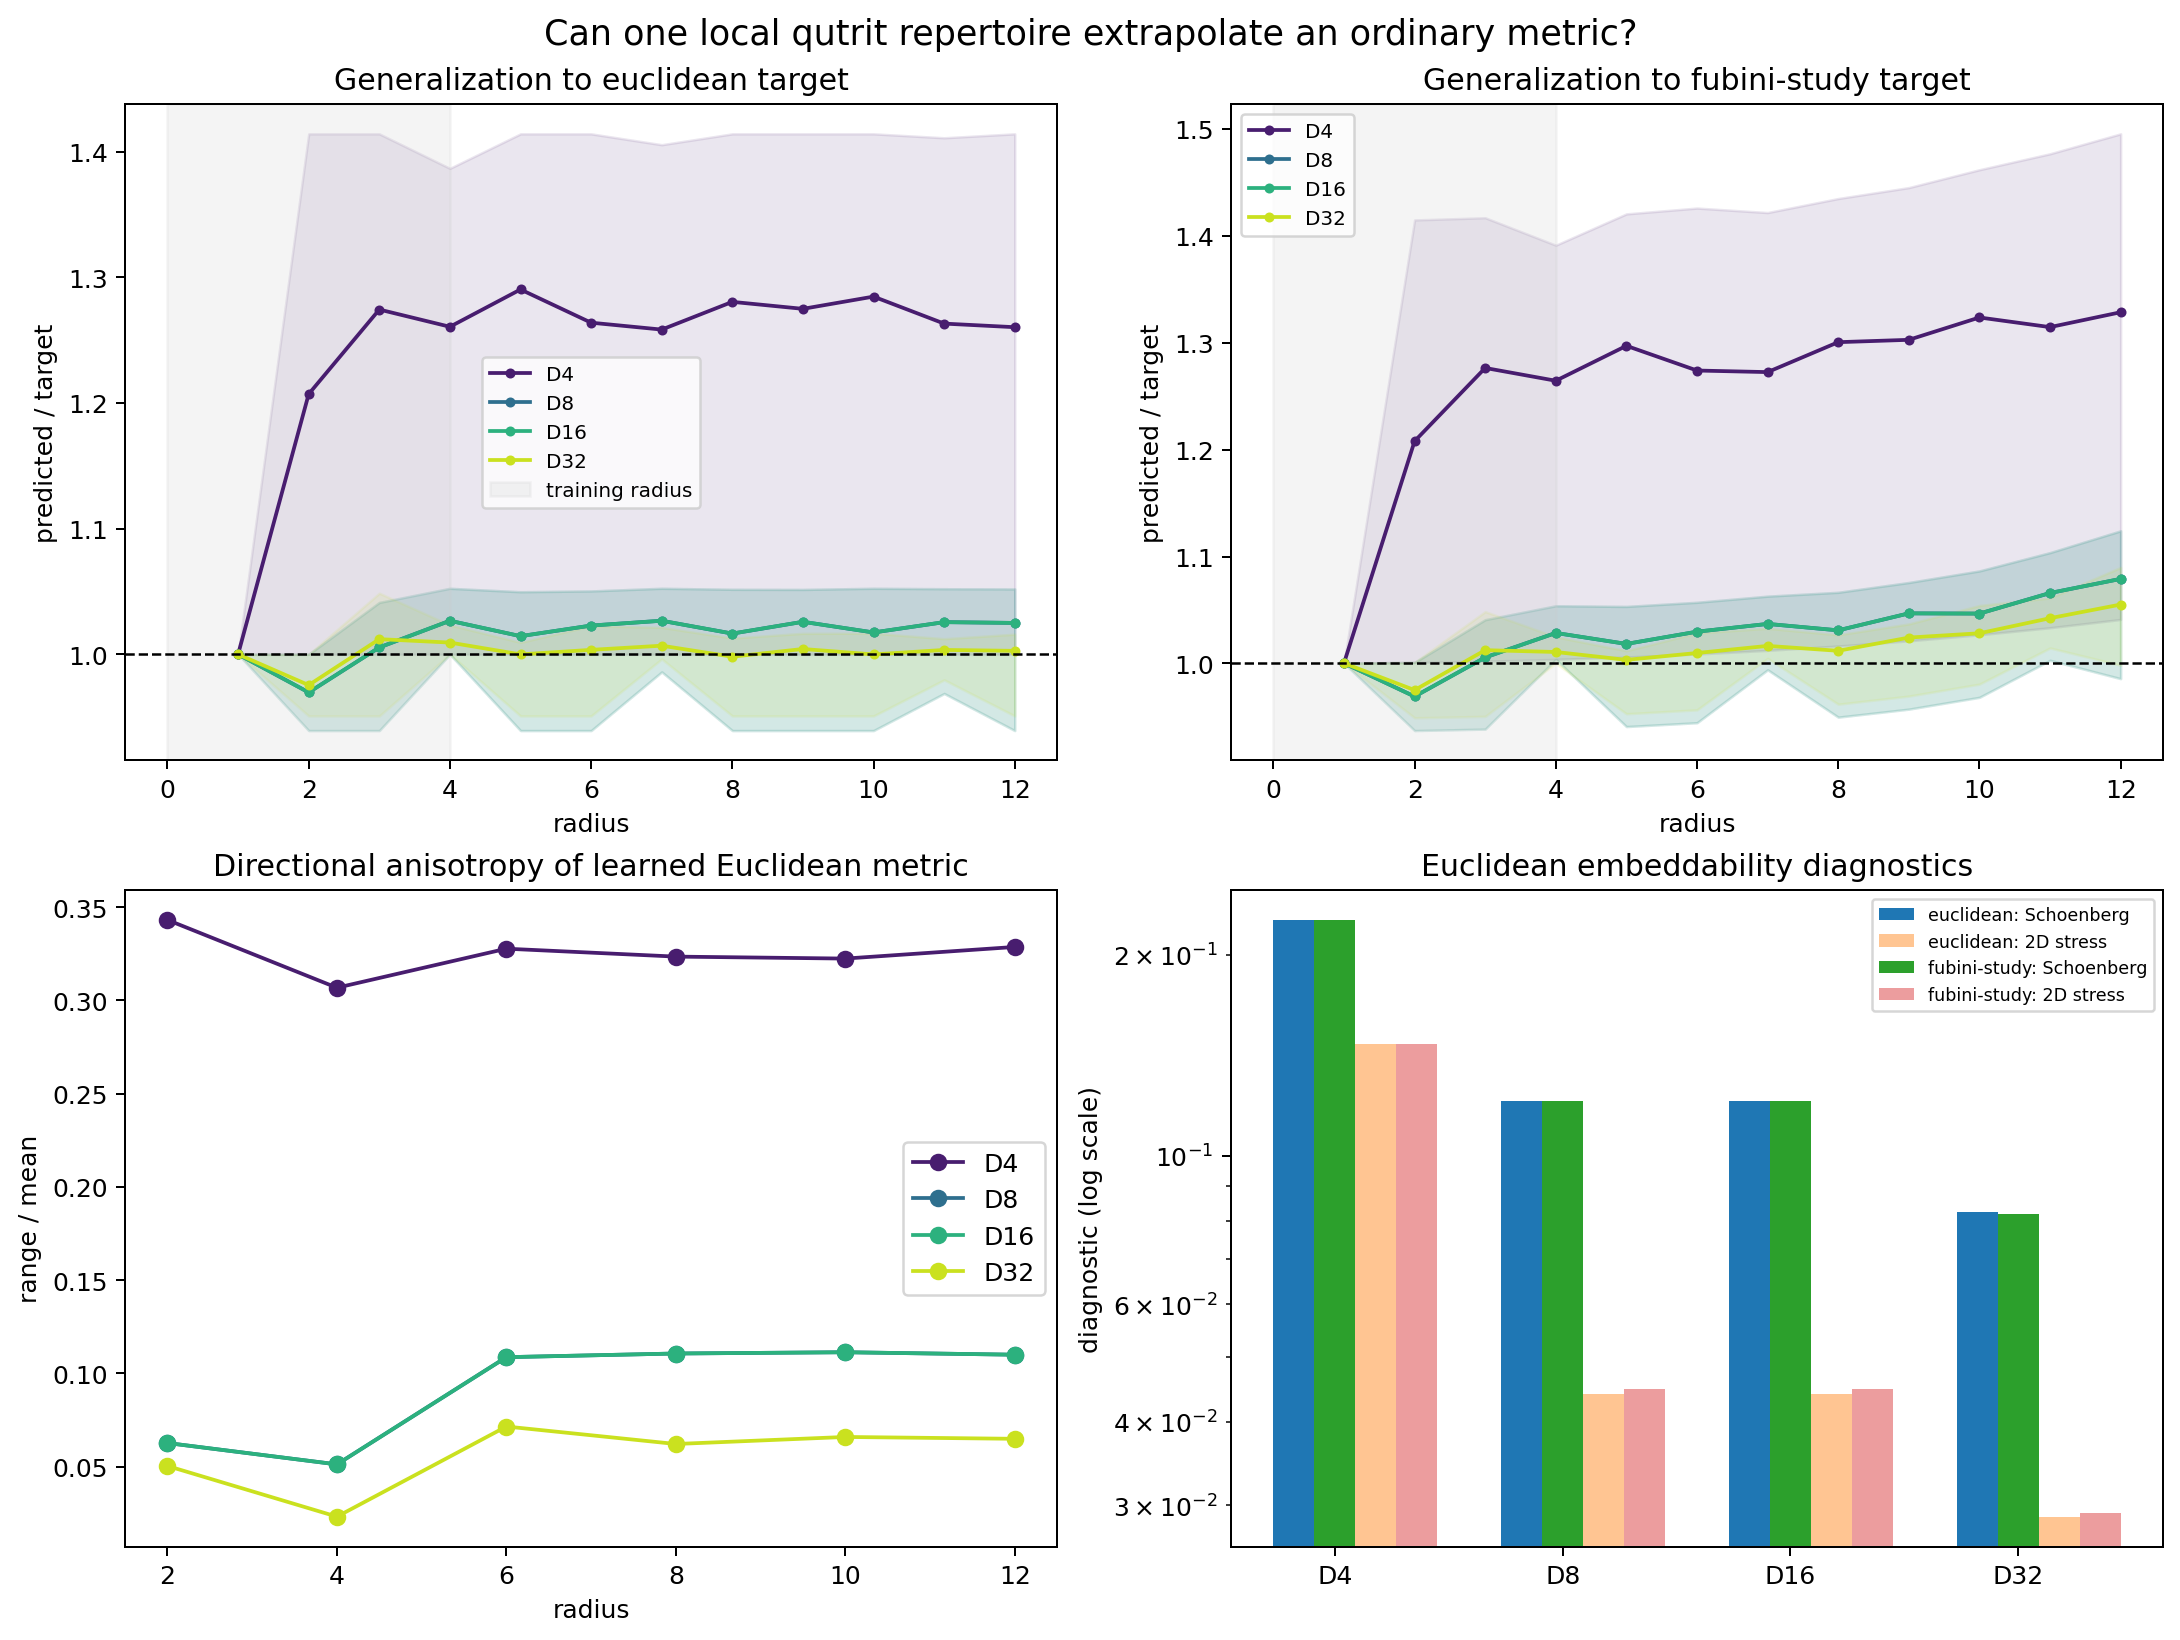
\includegraphics[width=\textwidth]{control/results/figures/local_control_summary.png}
\caption{Local-control results. Top: predicted-to-target ratios by radius for
Euclidean and scaled Fubini--Study targets. The gray region is fitted; larger
radii are held out. Shading is directional range, not uncertainty. Bottom:
anisotropy and Euclidean embeddability. More exposed directions improve the
geometry but do not make a finite catalog exactly Euclidean.}
\label{fig:control}
\end{figure}

At radius 12, directional range divided by mean is about \(0.329\) for D4,
\(0.110\) for D8/D16, and \(0.065\) for D32. On the 25-goal diagnostic patch,
Schoenberg negative-eigenmass falls from \(0.2254\) to \(0.1207\) and
\(0.08236\); 2D MDS stress falls from \(0.1469\) to \(0.04409\) and
\(0.02887\). D32 looks convincingly planar, yet the spectral test correctly
refuses an exact Euclidean interpretation.

\section{Hidden-start localization}
\label{sec:localization-theory}

\subsection{Why geometry alone is insufficient}

The control study assumes a known source, so the agent can integrate observed
successes. It tests the base metric but not access to position. A second model
therefore hides a uniformly sampled initial label and provides weak quantum
measurements. A finite \(\Z_3^2\) orbit permits exact filtering and analytic
controls.

Let \(\omega=e^{2\pi i/3}\) and
\begin{equation}
\ket{\phi_{xy}}=\frac{\ket0+\omega^x\ket1+\omega^y\ket2}{\sqrt3},
\qquad (x,y)\in\Z_3^2.
\label{eq:phase-grid}
\end{equation}
These nine states are not a basis. Distinct pairs have fidelity zero or
\(1/3\), and
\begin{equation}
\frac13\sum_{x,y}\proj{\phi_{xy}}=I_3.
\label{eq:frame}
\end{equation}
The commuting unitaries
\[
U=\operatorname{diag}(1,\omega,1),\qquad
V=\operatorname{diag}(1,1,\omega)
\]
translate the two labels modulo three. The moves
\(U,U^\dagger,V,V^\dagger\) have unit cost and give a toroidal Manhattan
metric. This model studies localization, not the Euclidean stencil fit.

\subsection{Weak covariant sensor}

For strength \(0\le\eta\le1\), outcome \(o\in\Z_3^2\) has effect and Lüders
Kraus operator
\begin{equation}
E_o(\eta)=\frac{\eta}{3}\proj{\phi_o}
+\frac{1-\eta}{9}I_3,\qquad K_o(\eta)=\sqrt{E_o(\eta)}.
\label{eq:weak-povm}
\end{equation}
The frame identity gives \(\sum_oE_o=I\). At \(\eta=0\), outcomes are uniform
noise and the normalized state is unchanged. At \(\eta=1\), the rank-one
phase POVM resets the state to the reported \(\ket{\phi_o}\). Intermediate
strength trades preparation information against disturbance
\cite{holevo2011,helstrom1976,wiseman2010}.

Each episode samples a label \(S\) uniformly and prepares \(\ket{\phi_S}\).
The label is a hidden laboratory record used to score ensemble discrimination,
not an ontic property of the average state:
\[
\bar\rho_0=\frac19\sum_s\proj{\phi_s}=\frac I3.
\]
The same mixed state admits many ensemble decompositions.

\subsection{Exact Bayesian quantum filter}

A classical likelihood table is wrong after the first observation because
backaction changes every hidden-preparation branch. The exact filter stores a
posterior weight \(w_s\) and conditional state \(\rho_s\) for each hypothesis.
For observed \(o\),
\begin{align}
\ell_s(o)&=\tr(E_o\rho_s),&
p(o)&=\sum_sw_s\ell_s(o),\\
w_s'&=\frac{w_s\ell_s(o)}{p(o)},&
\rho_s'&=\frac{K_o\rho_sK_o^\dagger}{\ell_s(o)}.
\label{eq:filter}
\end{align}
The present predictive state is
\begin{equation}
\bar\rho=\sum_sw_s\rho_s.
\label{eq:predictive}
\end{equation}
This nine-branch filter is the exact benchmark for a future learned recurrent
predictive representation.

\subsection{Two goals on the same history}

The experiment scores two criteria.
\begin{enumerate}[leftmargin=2em]
\item \textbf{Preparation-label navigation.} Let
\(\hat S=\arg\max_sw_s\). Apply the translation that would move \(\hat S\) to
goal \(g\). Label success means \(\hat S=S\).
\item \textbf{Present-state navigation.} Find the phase-grid projector with
greatest fidelity to \(\bar\rho\), translate that center to \(g\), and score
\(\bra{\phi_g}\rho_{\rm final}\ket{\phi_g}\).
\end{enumerate}
The first asks where the episode began; the second asks which action controls
the state that exists now. They coincide in a perfectly observed
nondisturbing classical register, but not here.

\begin{proposition}[One-shot information--preparation gap]
\label{prop:one-shot}
With a uniform preparation and one sensor outcome,
\begin{equation}
P(\hat S=S)=\frac{1+2\eta}{9},\qquad
F_g=\frac{1+2\eta}{3},
\label{eq:one-shot}
\end{equation}
where \(F_g\) is the final fidelity obtained by translating the reported
outcome to \(g\).
\end{proposition}
\begin{proof}
Since the predictive state is \(I/3\), every outcome has
\(p(o)=\tr(E_oI/3)=1/9\). The matching hypothesis has likelihood
\[
p(o\mid s=o)=\bra{\phi_o}E_o\ket{\phi_o}
=\frac{\eta}{3}+\frac{1-\eta}{9}
=\frac{1+2\eta}{9}.
\]
Symmetry makes it the MAP hypothesis, proving the first formula. The
conditioned ensemble state is
\[
\bar\rho_o=\frac{K_o(I/3)K_o}{1/9}
=3E_o=\eta\proj{\phi_o}+(1-\eta)\frac I3.
\]
Translating \(o\) to \(g\) yields fidelity
\(\eta+(1-\eta)/3=(1+2\eta)/3\).
\end{proof}

At \(\eta=1\), initial-label accuracy is only \(1/3\), while present-state
fidelity is one. The first sharp outcome erases all remaining quantum
dependence on the preparation. Later sharp outcomes contain no more
information about \(S\). Posterior entropy falls from
\(\log_2 9=3.169925\) bits to \(2.641604\) bits and then remains fixed.

\subsection{Policies and controls}

Fixed rules use \(0,1,3,\) or \(5\) observations. Adaptive rules stop when
\(\max_sw_s\) reaches \(0.25\), \(0.32\), or \(0.50\), with a six-sense cap.
Every sensor, move, and terminal commitment costs one. Covariance makes
translation before sensing a mere permutation of outcomes, so this first model
studies stopping rather than probe choice.

The null sensor \(\eta=0\) changes neither posterior nor state; hidden-label
success must remain \(1/9\). The known-start control uses no sensor and reaches
both terminal criteria exactly. Its uniform mean torus movement distance is
\(4/3\), so mean total cost including commitment is \(7/3\).

\section{Localization results}
\label{sec:localization-results}

\subsection{Protocol and representative results}

The production bundle contains 60,000 seeded episodes: five strengths, seven
sensing rules plus a known-start control, and 1,500 episodes per condition.
Eight tests cover POVM and Kraus completeness, covariance, null sensing, exact
one-shot formulas, physical filter updates, known-start navigation, and
reproducibility. The maximum discrepancy from the analytic one-shot formulas
over all strengths is \(0.0196\).

\begin{table}[p]
\centering
\caption{Representative localization outcomes. Label-policy fidelity moves
according to the origin MAP estimate; state-policy fidelity moves according to
the present predictive state.}
\label{tab:localization}
\small
\begin{tabular}{rrlrrrrr}
\toprule
\(\eta\)&senses&rule&label success&label fidelity&state fidelity&
mean senses&total cost\\
\midrule
0.0&0&none&0.105&0.328&0.328&0.00&1.00\\
0.0&5&fixed&0.099&0.325&0.325&5.00&6.00\\
0.2&1&fixed&0.147&0.459&0.459&1.00&3.33\\
0.2&5&fixed&0.189&0.548&0.553&5.00&7.32\\
0.5&1&fixed&0.203&0.659&0.659&1.00&3.34\\
0.5&5&fixed&0.271&0.735&0.786&5.00&7.36\\
0.5&--&adaptive 0.25&0.264&0.807&0.831&4.16&6.50\\
0.8&1&fixed&0.273&0.870&0.870&1.00&3.32\\
0.8&5&fixed&0.302&0.510&0.901&5.00&7.32\\
1.0&1&fixed&0.324&1.000&1.000&1.00&3.34\\
1.0&5&fixed&0.333&0.356&1.000&5.00&7.31\\
any&0&known start&1.000&1.000&1.000&0.00&\(\approx2.33\)\\
\bottomrule
\end{tabular}
\end{table}

\begin{figure}[p]
\centering
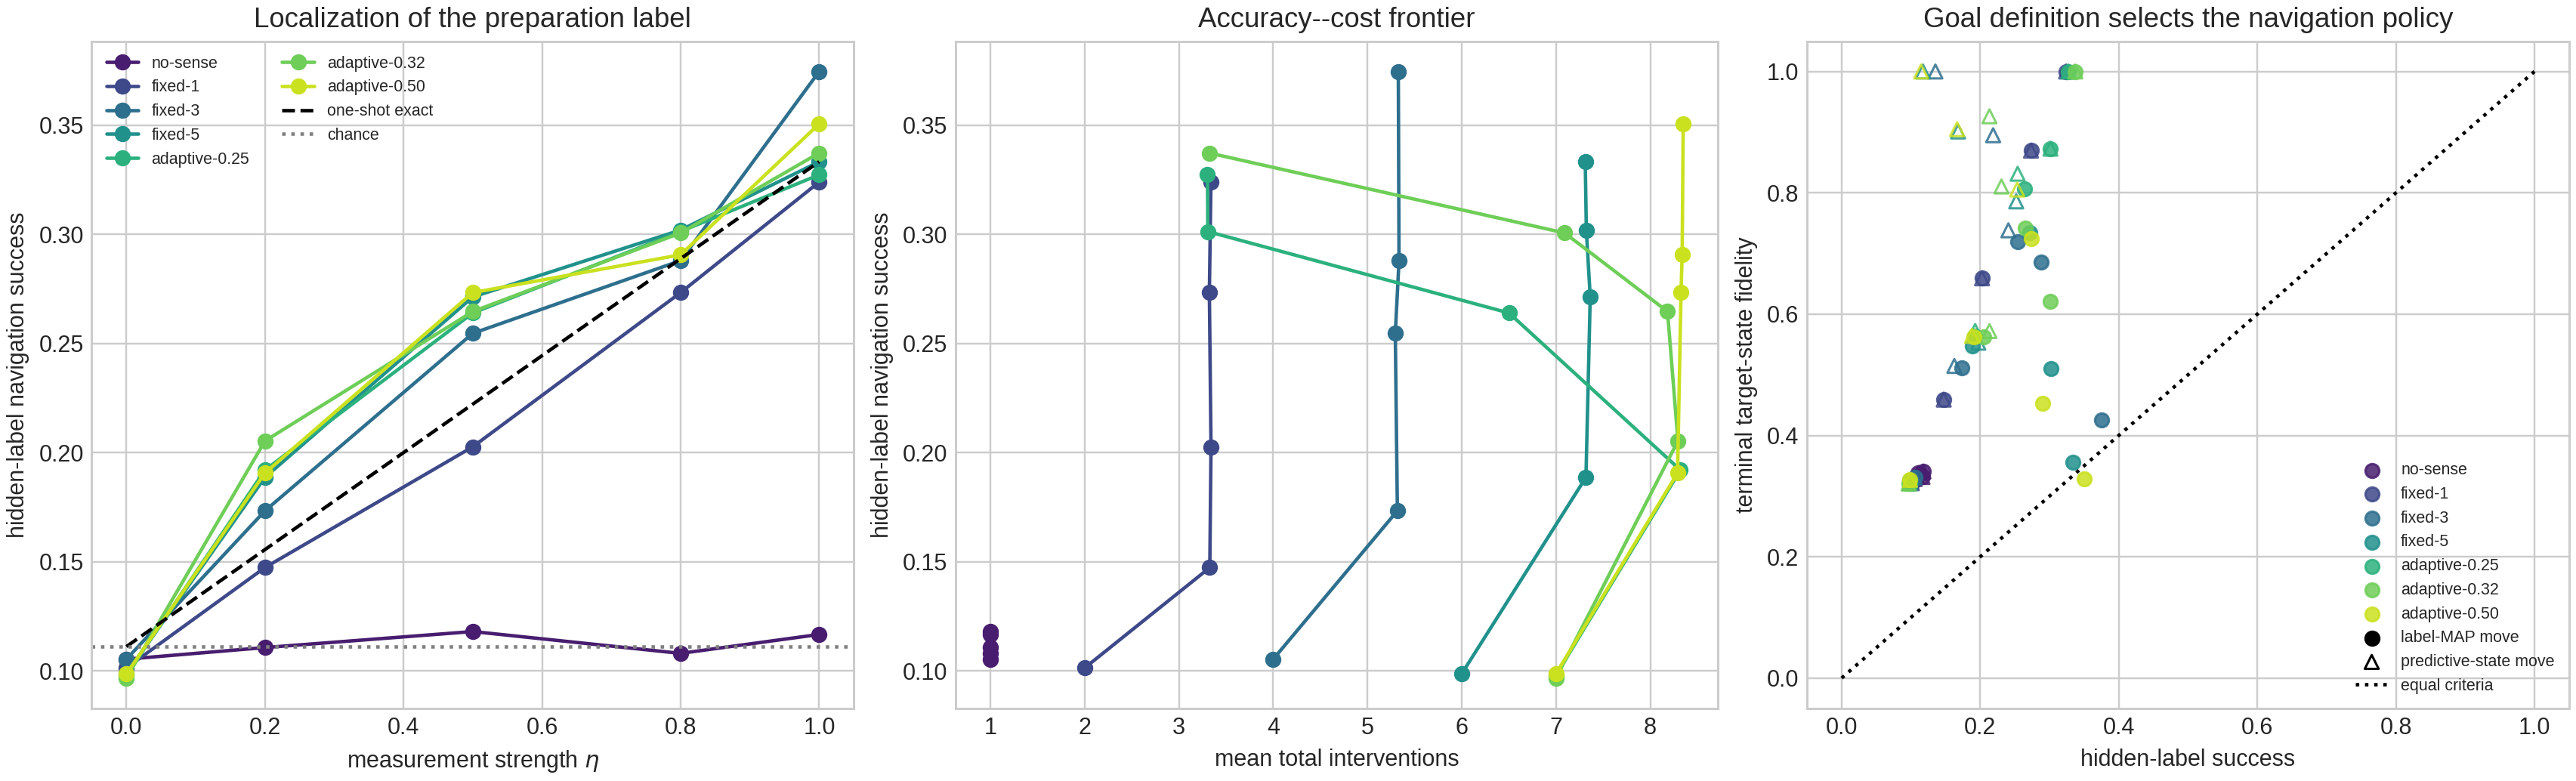
\includegraphics[width=\textwidth]{localization/figures/localization_performance.png}
\caption{Localization and control. Left: preparation-label success versus
strength. The dotted line is chance and the dashed line is the exact one-shot
formula. Center: label accuracy versus total cost. Right: terminal fidelity
versus label success. Filled circles use the historical-label move; hollow
triangles use the present-state move.}
\label{fig:localization-performance}
\end{figure}

At weak and medium strength, repeated observations accumulate origin
information. At \(\eta=0.5\), label success rises from \(0.203\) after one
observation to \(0.271\) after five, but total cost rises from \(3.34\) to
\(7.36\). The threshold-0.25 policy uses \(4.16\) observations, retains label
success \(0.264\), and reaches label-policy fidelity \(0.807\), better and
cheaper than fixed five.

At high strength, origin inference and present-state control diverge. At
\(\eta=0.8\), five observations raise label accuracy from \(0.273\) to
\(0.302\), yet historical-label fidelity falls from \(0.870\) to \(0.510\).
The predictive-state controller reaches \(0.901\). At \(\eta=1\), repeated
sensing cannot improve the origin posterior, but the predictive-state
controller retains unit fidelity by following the state prepared by the most
recent measurement.

\begin{figure}[p]
\centering
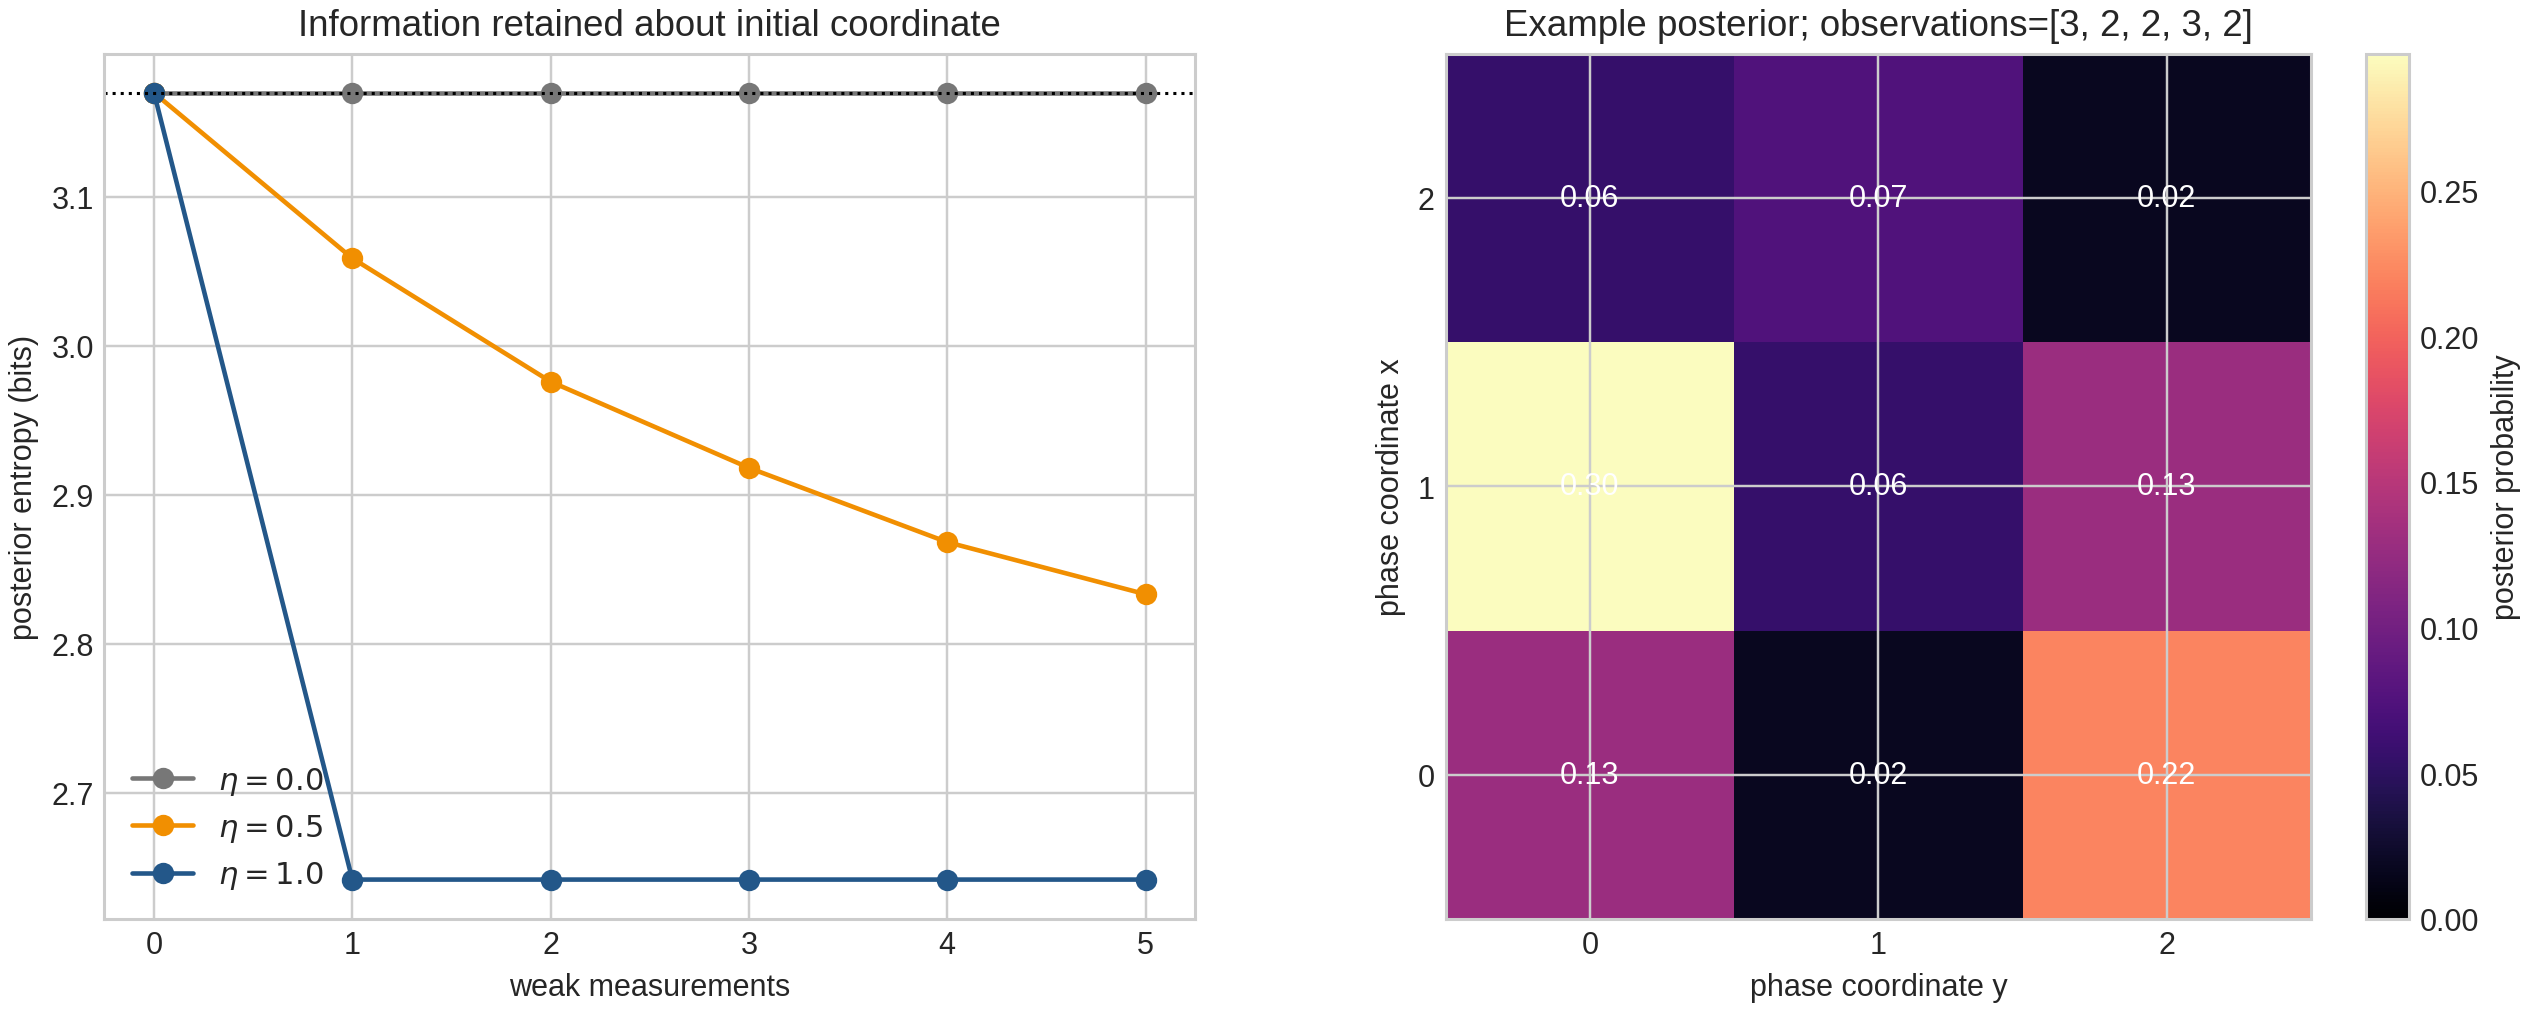
\includegraphics[width=\textwidth]{localization/figures/localization_beliefs.png}
\caption{Belief dynamics. Left: posterior entropy about the initial
coordinate. A sharp measurement extracts all retained origin information in
one step and then saturates; intermediate strength accumulates information.
Right: an example posterior after five outcomes. A point estimate cannot
represent the full operational state.}
\label{fig:localization-beliefs}
\end{figure}

Null sensing stays at chance and adds cost. Known-start motion is exact.
Informative sensing helps retrodiction but is limited by nonorthogonality and
backaction. These controls show that failure is neither broken movement nor
blind homing, and that measurement-induced preparation is not synonymous with
localization.

\section{Joint geometric interpretation}
\label{sec:interpretation}

\subsection{A Finsler base}

The control experiment identifies a homogeneous base action geometry whose
exact large-scale object is \(\norm{\cdot}_{P_S}\). D4 is Manhattan; D8 and
D32 are increasingly circular polygons. The base is spatial in locality,
translation covariance, and low-distortion planar embedding, but it is not
exactly Riemannian for a finite heading set.

The learned geometry is not ambient qutrit-ray distance. It is the Bellman
geometry of available transformations. Compact Hilbert-space recurrence can
coexist with an unbounded history-space covering coordinate.

\subsection{An epistemic quantum fiber}

With a hidden source, one coordinate is insufficient. Above a nominal phase
site lie posterior weights, hypothesis-conditioned density matrices, the
present ensemble state, and possibly sequence-goal automaton state.
Measurement transports this internal structure and changes which base point
best predicts future control. This resembles
\[
F_x\hookrightarrow E\xrightarrow{\pi}B,
\]
with movement geometry \(B\) and an epistemic/internal fiber \(F_x\).
It is not yet a mathematical fiber bundle: local trivializations, transition
functions, and a connection have not been established. It is an operational
precursor with measurable base--fiber coupling.

\subsection{Goal relativity}

The origin-MAP controller and predictive-state controller answer different
questions. If the goal is retrodiction, a newly prepared state is not success.
If the goal is present control, insisting on the origin can be harmful. Every
reported distance must specify the terminal criterion, cost convention,
available information, and whether it concerns history, current predictive
state, or a future outcome sequence. Their agreement in an orthogonal
classical position register is a special limit.

\section{Limitations}
\label{sec:limitations}

\begin{enumerate}[leftmargin=2em]
\item \textbf{Engineered primitive costs.} Goal-sized macro-actions are gone,
but primitive probabilities are still optimized against target geometry.
The study shows compositional extrapolation, not spontaneous selection of the
Euclidean norm.
\item \textbf{Finite headings.} The polygonal theorem guarantees a nonzero
anisotropy floor. D32 improves accuracy partly by extending primitive reach to
30\% of the evaluation radius.
\item \textbf{Two qutrit models.} Control uses a continuous equilateral phase
encoding; localization uses a finite \(\Z_3^2\) orbit. They share phase
translation structure but are not yet one end-to-end environment.
\item \textbf{Preparation label.} The hidden origin is a laboratory ensemble
record, not an intrinsic observable property of \(I/3\).
\item \textbf{Known filter.} The Bayesian model knows the instruments. A
recurrent agent has not learned the filter from trajectories.
\item \textbf{Limited active sensing.} One covariant sensor family makes
active design a stopping problem; inequivalent probes are absent.
\item \textbf{Statistics.} Control is deterministic. Localization is a
single recorded seed with 1,500 episodes per row, analytic checks, and
reported standard errors; multi-seed replication remains useful.
\item \textbf{No curvature yet.} The environments are homogeneous and
periodic or evaluated far from recurrence. There is no spatially varying
control tensor or demonstrated holonomy.
\end{enumerate}

\section{Continuous control and a predictive atlas}
\label{sec:outlook}

\subsection{Replace the polygon by a disk}

Let a qutrit have commuting phase generators \(A,B\) and continuous control
\begin{equation}
H(u)=u_1A+u_2B,\qquad \dot x=u.
\label{eq:continuous}
\end{equation}
If admissible velocities obey \(\norm u_2\le1\) and cost is elapsed time, the
velocity body is a disk and \(T^\star(x,g)=\norm{g-x}_2\). If instead
\(\abs{u_i}\le1\), it is a square and minimum time is Chebyshev. Euclidean
geometry is selected by isotropy of the resource body, not merely by two
coordinates.

\subsection{Quadratic effort and a metric tensor}

For fixed duration \(T\), define
\begin{equation}
\mathcal J[u]=\frac12\int_0^T u(t)^\top R(x_t)u(t)\,dt.
\label{eq:energy}
\end{equation}
For constant \(R\succ0\), Cauchy--Schwarz gives
\begin{equation}
\mathcal J^\star(x,g;T)=
\frac1{2T}(g-x)^\top R(g-x),
\label{eq:energy-opt}
\end{equation}
attained by constant velocity. The square root of
\(2T\mathcal J^\star\) is a flat Riemannian distance. Position-dependent
\(R(x)\) defines a curved metric and a Hamilton--Jacobi control problem
\cite{dalessandro2008}. This replaces hand-tuned retries with a physical
effort principle.

\subsection{Learn the predictive state}

The exact filter supplies scientific ground truth. A recurrent atlas should
receive only \((a_t,o_t)\) and learn
\[
z_{t+1}=F_\theta(z_t,a_t,o_t)
\]
that predicts next outcomes under contemplated interventions, goal-conditioned
cost, terminal fidelity, and calibrated operational uncertainty. Auxiliary
predictive likelihood is essential: a visually organized latent state is not
enough. Compare navigation regret, posterior calibration, held-out likelihood,
and latent probes directly with the exact filter.

\subsection{Genuine active localization}

Add rotated or coarse-grained phase POVMs so expected information gain depends
on the current posterior. The agent must choose whether to sense, which probe
to use, and measurement strength while accounting for disturbance. Small exact
belief-space dynamic programs provide oracle controls for learned
value-of-information policies.

\subsection{Base, fiber, and curvature tests}

Movement, sensing, and commitment should remain separate cost matrices.
Movement estimates the base; sensing estimates epistemic overhead. A total
cost can be useful for competence yet nonmetric. Calling its distortion
curvature would confound movement with information.

Once a stable base chart and learned internal state exist, transport the same
internal preparation around closed base loops. A reproducible loop-dependent
internal transformation, after controlling for base displacement and sensor
schedule, defines operational holonomy. Variation across nearby loops is the
first credible curvature observable. This is the appropriate bridge toward
bundle geometry, long before claims about general relativity.

\subsection{Falsifiers}

The next stage should be revised if rotational error does not decrease with a
continuous control disk; a recurrent latent cannot match exact posterior
calibration and predictive likelihood; apparent curvature vanishes when
sensing and movement costs are separated; loop transport has no reproducible
holonomy; or the geometry resides mainly in a hand-coded goal automaton rather
than outcome statistics.

\section{Conclusion}

Low Hilbert dimension is not the decisive obstruction to a large spatial goal
geometry. A qutrit supports many nonorthogonal phase goals, exact local
translations, and partial localization. The decisive geometric constraint is
the local control resource. A fixed finite heading catalog produces a
polygonal stable norm. It can approximate a plane impressively---D32 reaches
\(1.62\%\) held-out RMSE---but cannot become exactly rotationally invariant.

The localization study adds a second qualification. The place from which an
episode began and the move that controls the state now are different quantum
questions. Sharp sensing can prepare a perfectly controllable target while
retaining only \(1/3\) origin accuracy. Operational state therefore contains
a base coordinate and an internal posterior/quantum structure.

The strongest next model combines continuous isotropic qutrit control with a
learned predictive atlas. Position-dependent control effort and closed-loop
internal transport can then test metric curvature and connection. The present
proofs, controls, and calibrated simulations provide the baseline required to
distinguish genuine emergence from geometry inserted by hand.

\appendix
\section{Stable-norm duality and active actions}

The gauge has the linear program
\[
\norm x_{P_S}=\inf_{\alpha_v\ge0}
\left\{\sum_v\alpha_v\ell_v:\sum_v\alpha_vv=x\right\}
\]
and dual
\[
\norm x_{P_S}=\sup_{\xi\in\R^2}
\left\{\xi\cdot x:\xi\cdot v\le\ell_v\text{ for all }v\right\}.
\]
An action affects the asymptotic metric only if \(v/\ell_v\) is an exposed
point of \(P_S\). This makes the D16 failure predictable: an action inside the
D8 hull cannot change the gauge. Randomized policies fill \(P_S\) by convex
mixtures but cannot curve its boundary.

General noisy increments can add diffusion corrections. An isotropic heat
kernel may define a Riemannian metric through a Varadhan-type relation
\[
d_g(x,y)^2=\lim_{t\downarrow0}-4t\log p_t(x,y)
\]
\cite{varadhan1967}. This is not expected hitting time. In two dimensions an
unbiased infinite random walk is recurrent but has infinite mean point-hitting
time. Diffusion geometry is promising, but changes the operational definition
and must be studied explicitly.

\section{Statistical formulas}

For \(N\) primitive surveys,
\[
\operatorname{SE}(\hat p)\approx\sqrt{\frac{p(1-p)}N}.
\]
With \(\ell=1/p\), the delta method gives
\[
\frac{\operatorname{SE}(\hat\ell)}\ell
\approx\sqrt{\frac{1-p}{Np}}.
\]
Learned geometry should approach the exact polygonal model at
\(N^{-1/2}\), not cross its structural anisotropy floor. Binomial navigation
standard errors use
\(\sqrt{\hat q(1-\hat q)/N}\); fidelity standard errors use sample standard
deviation divided by \(\sqrt N\).

\section{Reproducibility}

From the repository root:
\begin{verbatim}
python -m unittest discover \
  -s low_dimensional_hodology/emergent_local_metric/control/tests -v
MPLBACKEND=Agg python \
  low_dimensional_hodology/emergent_local_metric/control/run_local_control.py

python -m unittest discover \
  -s low_dimensional_hodology/emergent_local_metric/localization \
  -p 'test_*.py' -v
MPLBACKEND=Agg python \
  low_dimensional_hodology/emergent_local_metric/localization/\
  localization_experiment.py --episodes 1500 --seed 20260811
\end{verbatim}
Control artifacts include optimized costs, held-out displacements, anisotropy,
diagnostics, and the summary figure. Localization artifacts include full
condition summaries, posterior calibration, exact one-shot predictions,
representative episodes, a manifest, and both figures. The two strands contain
15 focused tests.

\begin{thebibliography}{99}
\bibitem{bellman1957} R.~Bellman, \emph{Dynamic Programming}, Princeton
University Press (1957).
\bibitem{puterman1994} M.~L. Puterman, \emph{Markov Decision Processes},
Wiley (1994).
\bibitem{sutton2018} R.~S. Sutton and A.~G. Barto,
\emph{Reinforcement Learning: An Introduction}, 2nd ed., MIT Press (2018).
\bibitem{kaelbling1998} L.~P. Kaelbling, M.~L. Littman, and A.~R. Cassandra,
Planning and acting in partially observable stochastic domains,
\emph{Artificial Intelligence} \textbf{101}, 99--134 (1998).
\bibitem{littman2002} M.~L. Littman, R.~S. Sutton, and S.~Singh,
Predictive representations of state, in \emph{Advances in Neural Information
Processing Systems 14}, 1555--1561 (2002).
\bibitem{kraus1983} K.~Kraus, \emph{States, Effects, and Operations},
Springer (1983).
\bibitem{nielsen2010} M.~A. Nielsen and I.~L. Chuang,
\emph{Quantum Computation and Quantum Information}, Cambridge University
Press (2010).
\bibitem{wiseman2010} H.~M. Wiseman and G.~J. Milburn,
\emph{Quantum Measurement and Control}, Cambridge University Press (2010).
\bibitem{holevo2011} A.~S. Holevo,
\emph{Probabilistic and Statistical Aspects of Quantum Theory}, 2nd ed.
(2011).
\bibitem{helstrom1976} C.~W. Helstrom,
\emph{Quantum Detection and Estimation Theory}, Academic Press (1976).
\bibitem{bengtsson2017} I.~Bengtsson and K.~Zyczkowski,
\emph{Geometry of Quantum States}, 2nd ed., Cambridge University Press (2017).
\bibitem{schoenberg1935} I.~J. Schoenberg, Remarks to Maurice Frechet's
article on Hilbert-space distance, \emph{Annals of Mathematics}
\textbf{36}, 724--732 (1935).
\bibitem{kruskal1964} J.~B. Kruskal, Multidimensional scaling by optimizing
goodness of fit, \emph{Psychometrika} \textbf{29}, 1--27 (1964).
\bibitem{borg2005} I.~Borg and P.~J.~F. Groenen,
\emph{Modern Multidimensional Scaling}, 2nd ed., Springer (2005).
\bibitem{bao2000} D.~Bao, S.-S. Chern, and Z.~Shen,
\emph{An Introduction to Riemann--Finsler Geometry}, Springer (2000).
\bibitem{burago2001} D.~Burago, Y.~Burago, and S.~Ivanov,
\emph{A Course in Metric Geometry}, AMS (2001).
\bibitem{varadhan1967} S.~R.~S. Varadhan, Diffusion processes in a small time
interval, \emph{Communications on Pure and Applied Mathematics}
\textbf{20}, 659--685 (1967).
\bibitem{dalessandro2008} D.~D'Alessandro,
\emph{Introduction to Quantum Control and Dynamics}, CRC Press (2008).
\end{thebibliography}

\end{document}
